\subsection{MIS Capacitance Structure}\label{sec:mis_capacitance_structure}

We are now reaching the last part of what we need to understand in physics before getting to the transistor.
The \textit{Metal-Insulator-Semiconductor} (MIS) structure consists of assembling conductor and a semiconductor that are separated by a thin insulator layer. The most common version of the MIS structure is the MetalOxide-Silicon (MOS) structure, where the ‘oxide’ is in most cases silicon dioxide ($SiO_2$). The MOS structure and the PN junction diode are the building blocks of today’s most widely used type of transistor, commonly known as Metal-Oxide-Semiconductor Field-Effect Transistor (MOSFET). This is the transistor we will study in the next chapter. 

\begin{figure}[H]
    \centering
    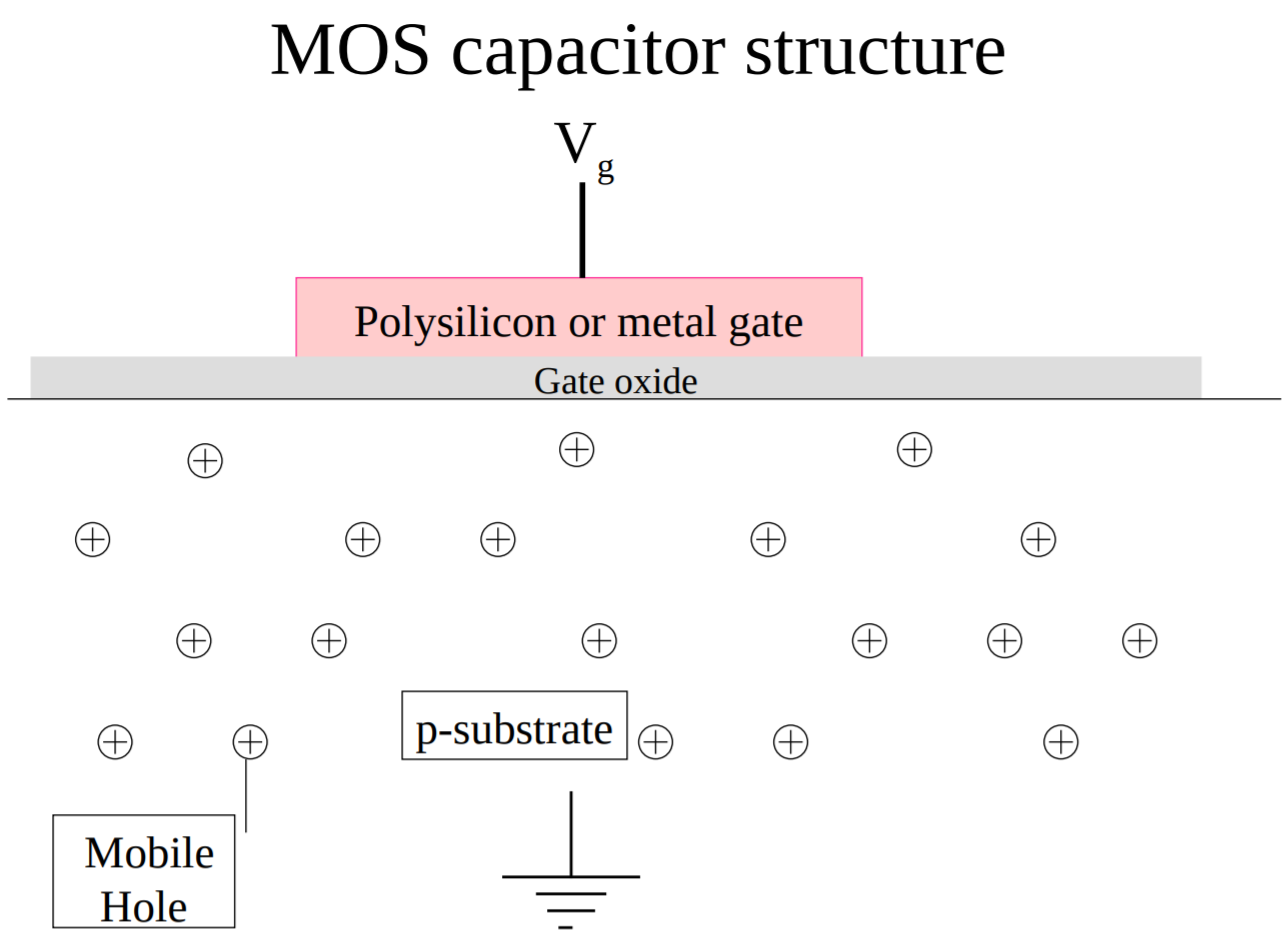
\includegraphics[width=0.6\linewidth]{../../Figures/MOS Structure.PNG}
    \caption{MOS Capacitor structure. A thin layer of insulating \textit{Gate Oxide} separates two conductive material: a polysilicon metal gate and a doped semi conductor \textit{p substrate}. Adapted From Lecture Notes.}
    \label{fig:MOS Structure}
\end{figure}

As shown in figure \ref{fig:MOS Structure}, a thin layer of insulating \textit{Gate Oxide} separates two conductive material: a polysilicon metal gate and a doped semi conductor \textit{p substrate}. The p-substrate is simply p-doped silicon, which is at a potential of $0V$ in this case, as can be seen on the figure (it is connected to ground). Because of the capacitive structure, interesting things start to happen when we apply a non-zero voltage on the metal gate, which is what we need to look at. Typically, imagine that when applying a negative voltage on the metal gate, negative charges accumulate on the gate and positive charges accumulate on the other side of the insulating layer in the p-substrate. Conversely, when applying a positive voltage on the gate, positive charges accumulate on the gate and negative charges accumulate on the surface of the insulating layer of the p-substrate. Essentially, very distinct dynamics are obtained as a function of the applied gate voltage - this is critical to understand the transistor. Let's look at all the different case scenarios and their implications \footnote{We'll only take the example of p-substrate, but the inverse holds when working in n-substrate.}: 

\begin{figure}[H]
    \centering
    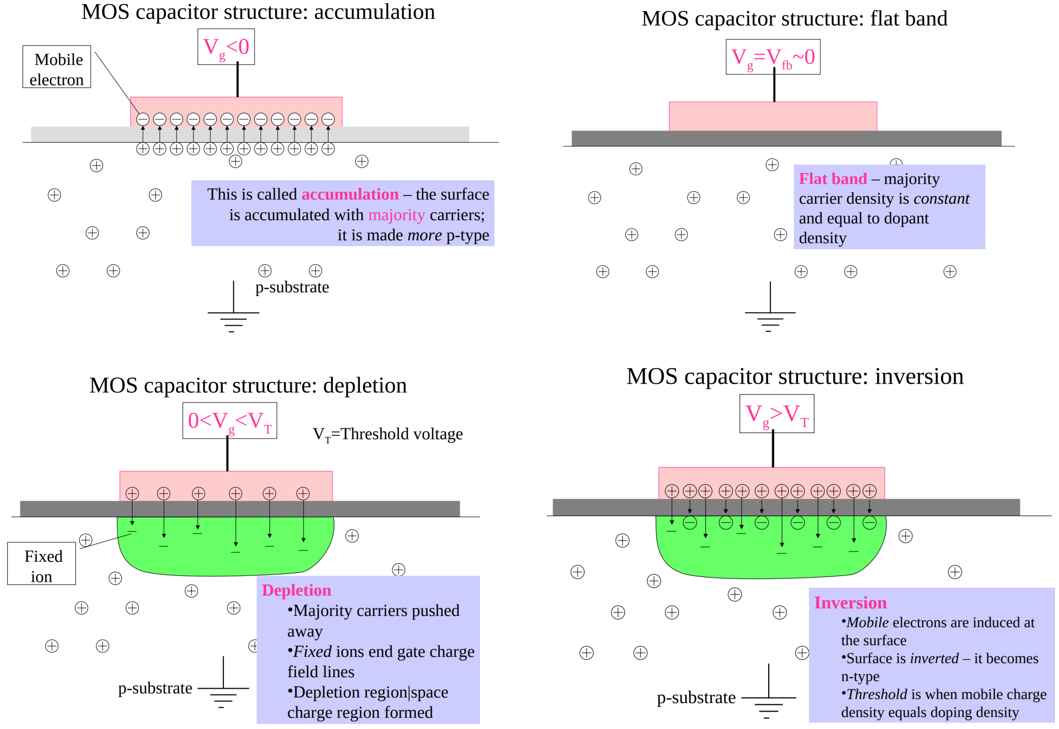
\includegraphics[width=1\linewidth]{../../Figures/MOS_Capacitance.PNG}
    \caption{MOS Capacitance and its different operation modes. Adapted From Lecture Notes.}
    \label{fig:MOS_Capacitance}
\end{figure}

\paragraph{Accumulation}

Accumulation happens when a charge on the gate attracts a lot of \textbf{majority} carriers on the surface of the semiconductor underneath it. For a p-substrate channel (as shown in figure \ref{fig:MOS_Capacitance}), a negative voltage on the gate means mobile electrons on the gate. These electrons attract positive charges on the semiconductor surface underneath it, leading to accumulation of them. Since positive charges (holes) are the majority carrier in p-substrate, we call this situation accumulation. 

\paragraph{Flat Band}

In an ideal MIS diode, with no bias applied, the work function of the metal and the semiconductor are the same. The Fermi levels line up and the energy bands in the semiconductor are flat. Flat-Band Condition
With $V_g = 0$, the majority carrier density is constant and equal to the dopant density.

\paragraph{Depletion}

For a p-substrate channel, if we apply a positive subthreshold voltage on the gate (positive charges), we push away positive majority carriers on the semiconductor surface. A depletion region is created where only \textbf{fixed} negative charge carriers remain. This is the same depletion region we saw in the PN-Junction; but instead of being formed naturally, you create it by pushing the majority carriers of the p-substrate away. 

\paragraph{Inversion}

Eventually, by increasing the positive voltage on the gate and pushing away majority carriers from the p-substrate away from the gate, we start having \textbf{mobile} minority carriers (electrons here) accumulating at the semiconductor surface - this is called \textit{inversion}. Inversion happens when the surface is inverted: \textit{it becomes n-type silicon rather than p-type.} The precise gate potential at which this happens is known as the \textbf{threshold voltage} and is what distinguishes depletion from inversion mode. The threshold voltage is thus the exact voltage value at which mobile charge density equals doping density - when we go beyond, mobile charge takes over! \\

These dynamics are summarized in the following figure: 

\begin{figure}[H]
    \centering
    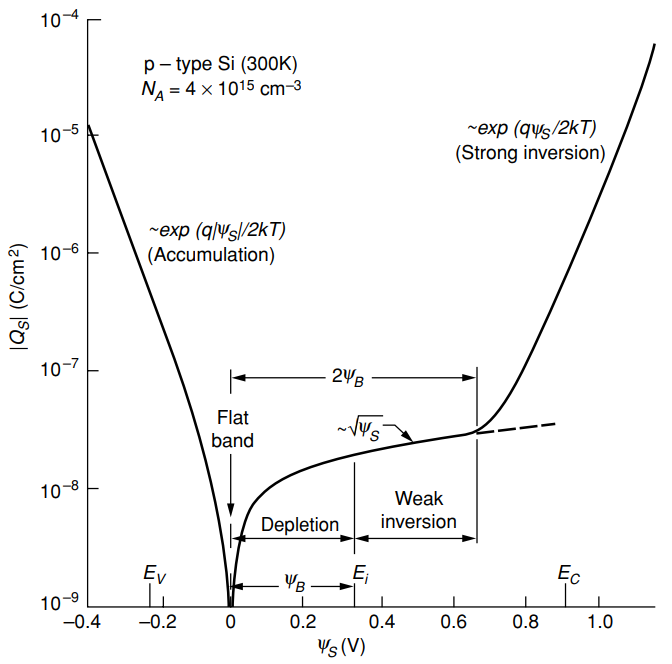
\includegraphics[width=0.6\linewidth]{../../Figures/Surface_Potential_MOS.PNG}
    \caption{Dependence of the area charge $Q_s$ on the surface potential for p-type silicon with acceptor density $N_A = 4 x10^{15} cm3$ at room temperature. Adapted From Textbook.}
    \label{fig:Surface_Potential_MOS}
\end{figure}

What one should pay attention to in this figure is how the surface potential changes as a function of $Q_s$. $Q_s$ is simply $-Q_g$, which is, like $Q_g$, directly related to the gate voltage $V_g$. Of course, this dependance varies with different doping concentration and other such factors, but the nature of the relationship remains the same. Now we can even draw some equation to summarize this point: 

\begin{equation}
    Q_g = - Q_s = Q_d + Q_i
\end{equation}

With $Q_d$ charge on the depletion layer and $Q_i$ charge on the inversion layer. Essentially, this yield a sort of capacitive model - the MIS Capacitance Structure - where we can consider charge at different points in the structure, and distinguish two capacitors: one actual one with the gate and the inversion region, and another virtual one between the depletion region and the substrate. We can say that the one between the depletion region and substrate is virtual as there is no actual insulators between the two charged regions, but there clearly are opposite charges on both ends, just like a capacitor. 

All the important elements subsequent from what we've just described are presented in the following 4 slides, which are shown on figure \ref{fig:MIS_Capacitance_Slides}. 

\begin{figure}[H]
    \centering
    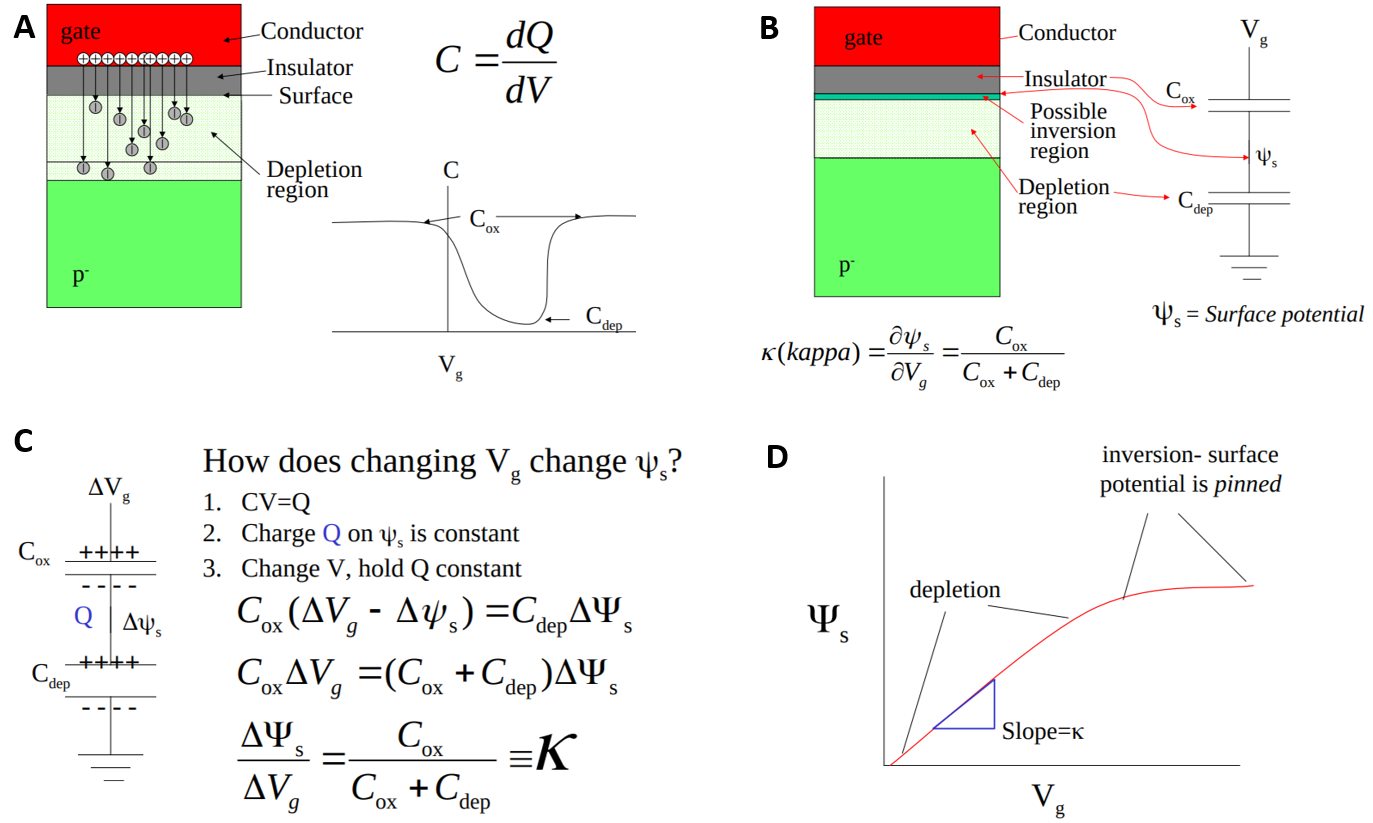
\includegraphics[width=1\linewidth]{../../Figures/MIS_Capacitance_Slides.PNG}
    \caption{A) The depletion capacitor. B) Influence of the gate on the surface potential. C) How does changing $V_g$ change $\psi_s$. D)  Change in $\kappa$ below and above threshold. Adapted From Lecture Notes.}
    \label{fig:MIS_Capacitance_Slides}
\end{figure}

Let's unpack all of this. 

\paragraph{A) The depletion capacitor} Let's remind ourselves that $C = \frac{dQ}{dV}$. This means that the more charge is accumulated per change in voltage, the higher the capacitance. We've described in the depletion regime that mobile charges are \textbf{pushed away}, only to leave \textbf{fixed ions}. This means that capacitance is \textbf{reduced} in the depletion regime! This justifies the graph we see on \ref{fig:MIS_Capacitance_Slides}.A. Now when we go above the threshold voltage, in inversion regime, remember that the voltage is so strong that mobile charge carriers are attracted to the surface. Change in voltage yields important change in charge carriers: capacitance is big again! We subsequently differentiate between Oxyde capacitance $C_{ox}$ and depletion capacitance $C_{dep}$.

\paragraph{B) Influence of the gate on the surface potential} On this figure, we see the full idea of the MIS capacitance structure, with the gate voltage, the oxyde capacitance, the surface potential, the depletion capacitance and the substrate - connected to ground. The surface potential changes as a function of the gate voltage - we define the change in surface potential $\psi_s$ as a function of the change in gate voltage with a value of important significance: $\kappa$. 
\begin{equation}
    \frac{d\psi_s}{dV_g} = \frac{C_{ox}}{C_{ox} + C_{dep}} =  \kappa
\end{equation} 

Because this rate of change is different depending on the operating regime (depletion or inversion), it will have a different value as a function of the region. We will see this clearly in \ref{fig:MIS_Capacitance_Slides}.D. The math behind this will also become clearer in \ref{fig:MIS_Capacitance_Slides}.C.

\paragraph{C) How does changing $V_g$ change $\psi_s$} Here, we are trying to understand the equation derived previously, that is, why $\frac{d\psi_s}{dV_g} = \frac{C_{ox}}{C_{ox} + C_{dep}}$. The basic assumption to understand this is that the charge doesn't change: whatever charge appears on $C_{ox}$ need also be on $C_{dep}$, simply because of charge conservation. No charge can be created! From this, understanding the equation on the figure is (relatively) straightforward. 
Now one intuition to remember: if $C_{ox}$ is big, $\kappa$ will be close to 1

\paragraph{D) Change in $\kappa$ below and above threshold} $\kappa$ is the slope of $\psi_s$ vs $V_g$! It is constant below threshold and experiences a shift when approaching the threshold to become again constant, and close to 0, above threshold. This is because, in inversion, the surface potential is pinned - so the change in surface potential is very small when changing gate voltage. 

\paragraph{Concluding thoughts on MIS Capacitance}\\

If this is not perfectly clear for you, you're not alone - this is one of the trickiest concept about device physics and really the whole module. It also happens to be one of the most important one to understand transistors dynamics. The issue is that abstractions and simplifications have limits: the dynamics described here are very complex and need substantial physics to understand clearly. But because this really is not the topic of Neuromorphic Engineering, it is taught rather quickly. In any case, there are some absolutely critical points that you should remember and be fairly okay with about this: 

\begin{itemize}
    \item What MIS Capacitance stands for
    \item How changing the voltage at the gate influences what happens in the semiconductor substrate on the other side of the insulating layer
    \item Qualitatively describe the difference between Accumulation, Flat Band, Depletion and Inversion Regimes. 
    \item Understand the very important concept of the threshold voltage, and what specifically happens when we cross this threshold. 
    \item The two different capacitors in the MIS Capacitance: Oxyde capacitor and Depletion Capacitor 
    \item The idea behind $\kappa$, and how it relates surface potential to gate voltage (equations + slope).
\end{itemize}